%!TEX root = ../main.tex
\subsection{Methods to implement CAN on Linux}\label{sec:methods_to_implement_can}

\martin{The can controllers do not have anything to do with xilinux. Does Xilinux provide drivers for the can controllers on the zynq? CAN controllers vs CAN drivers Issue - Some things rephrased.}
After testing the stack board and showing the basic functionality of the CAN network as described in section \ref{sub:TestingCANStack_BareMetal}, the next step was to implement it using Linux running on the Zybo board.\\
Using Linux was necessary because the available sensors, GPS and IMU, as well as the WiFi dongle required an USB interface and the WiFi node needed various networking tools only present on a Linux operating system.
The process of establishing a wireless communication is explained in section \ref{sec:wifi}.
An operating system was also required for logging purposes, specifically to log data into files.
This section describes the necessary procedures that were followed in order to gain control over the CAN network from Linux.
The different approaches that were explored, described in the next section, include:
\begin{itemize}
\item utilizing the XCanPs
\item utilizing the AXI CAN IP Core
\item implementing asymmetric multiprocessing.
\end{itemize}
~\\
At this point the reader should be informed that although the CAN controllers could be used on the Processing System using bare-metal code, the implementation of CAN on the Programmable Logic and the access to it from Linux was not successful.
After a lot of effort to create a physically functional network and researching on how to implement it, the conclusion that the available documentation is lacking was reached.
Alternatively, other means to prove the concept of the project were taken into account, as described in section \ref{sub:Utilizing_Svr_Virtualization}.

\subsubsection{Enabling the CAN Controller Drivers}

This was the first idea on how to utilize the CAN network using Linux.
In order to gain access to the CAN controllers on the Zynq7 Processing System, the Linux CAN driver guide \cite{Xilinx_wiki_Linux_CAN_driver} was followed in order to enable the necessary drivers.
The Kconfig file under the path \ref{code:can_kconfig_pathfile} needed to be configured.
The entry at line 128 was changed as seen in the code snippet \ref{code:can_kconfig_contents_line128}.
Originally, lines 130 and 131 were as seen in the snippet \ref{code:can_kconfig_original_line130}.

\begin{lstlisting}[caption={CAN Kconfig pathfile.},numbers=none,label=code:can_kconfig_pathfile]
/usr/src/kernels/3.12.0-xillinux-1.3/drivers/net/can
\end{lstlisting}

\begin{lstlisting}[firstnumber=128,caption={Kconfig file contents from line 128.},label={code:can_kconfig_contents_line128}]
config CAN_XILINXCAN
	tristate "Xilinx(*@ @*)CAN"
	depends on NET [=y] && CAN_DEV [=y] && CAN [=y] && (ARCH_ZYNQ ||
		MICROBLAZE [=y])
	default y
	---help---
	  Xilinx CAN driver. This driver supports both soft AXI CAN IP
	  and Zynq CANPS IP.
\end{lstlisting}

\begin{lstlisting}[firstnumber=130,caption={Original content of lines 130 and 131.},label={code:can_kconfig_original_line130}]
	depends on CAN && (ARCH_ZYNQ || MICROBLAZE)
	default n
\end{lstlisting}

The next step of the process was the modification of the device tree settings file, requiring an entry for the CAN PS to be inserted.
The necessary file was located under the boot folder named as seen in \ref{code:dts_file_zybo}.
The modifications can be seen in the snippet \ref{code:dts_changes_zybo} for can controllers as well as for the AXI CAN core.

\begin{lstlisting}[numbers=none,caption={Device tree settings file and its path.},label={code:dts_file_zybo}]
/boot/xillinux-1.3-zybo.dts
\end{lstlisting}
\catalin{Double quotes are problem here as well. FIX THEM WHENEVER}
\begin{lstlisting}[caption={Device tree settings changes.},label={code:dts_changes_zybo}]
zynq_can_0: can@e0008000 {
        compatible = xlnx,zynq-can-1.0;
        clocks = <&clkc 19>, <&clkc 36>;
        clock-names = can_clk, pclk;
        reg = <0xe0008000 0x1000>;
        interrupts = <0 28 4>;
        interrupt-parent = <&intc>;
        tx-fifo-depth = <0x40>;
        rx-fifo-depth = <0x40>;
    };
axi_can_0: axi-can@40000000 {
        compatible = xlnx,axi-can-1.00.a;
        clocks = <&clkc 0>, <&clkc 1>;
        clock-names = can_clk,s_axi_aclk;
        reg = <0x40000000 0x10000>;
        interrupt-parent = <&intc>;
        interrupts = <0 59 1>;
        tx-fifo-depth = <0x40>;
        rx-fifo-depth = <0x40>;
        };
\end{lstlisting}

\mikkel{Maybe you can provide some thoughts about the problem. Maybe also some words about the patching Xilinx-Digilent etc.}
As was previously mentioned, the implementation was unsuccessful. At the time, the research done on this topic did not lead to successfully enabling the drivers.

\subsubsection{Utilizing the AXI CAN IP Core}

Another way to implement a CAN network was to use the AXI CAN core that is available in the Vivado Suite, instead of utilizing the CAN controllers on the Zynq chip.
Unfortunately due to a license restriction from Xilinx, the core can only be used for simulation purposes and not actual hardware implementations.
This information became available after the process of generating the bistream file in the form of an error, thus not allowing for further use of the core.
%The architecture can be seen in figure \ref{fig:CAN_Arch_with_AXI_CAN}.

%\begin{figure}[h!]
%	\centering
%	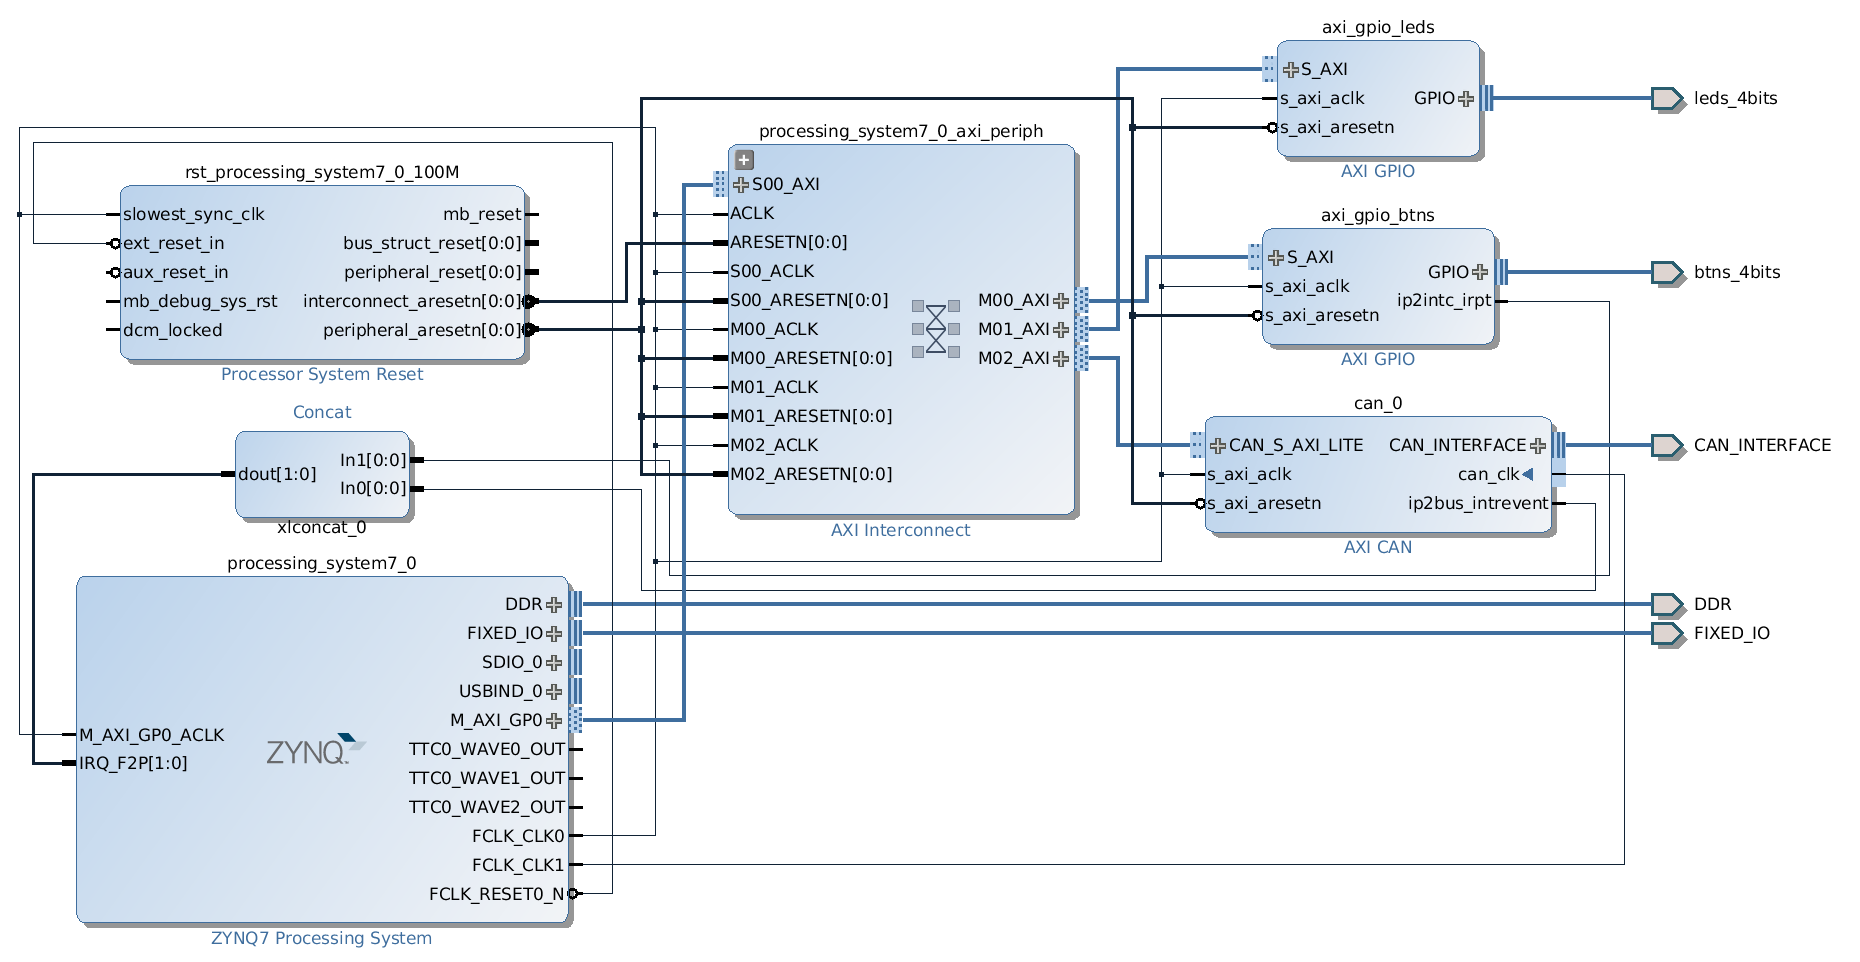
\includegraphics[width = 1.2\linewidth]{graphics/Zybo_Arch_with_AXI_CAN.png}
%	\caption{Block diagram featuring the architecture in Vivado with the AXI CAN core.}
%	\label{fig:CAN_Arch_with_AXI_CAN}
%\end{figure}

\subsubsection{Utilizing Asymmetric Multiprocessing}

Apart from using the AXI CAN core and the CAN drivers, the Zynq-7000 AP SoC provides the possibility of implementing a mechanism called asymmetric multiprocessing since there are two processors which share common memory as well as peripherals.
The idea of this is to run Linux OS on one processor, while on the other one a bare-metal system, which both of them can communicate with each other.
This was a proposed solution for the problem of accessing the CAN controllers from Linux which was the most promising of the implementation methods discussed in this report, but due to lack of time, it was researched only at a theoretical level.
\\
A brief implementation description will be given in this section, but for more details about the instructions and applications, the reader may refer to the Xilinx document \cite{Xilinx_AMP}.

\paragraph{Short Implementation Description}~\\
In order to achieve asymmetric multiprocessing on the Zybo board, certain steps are required to be taken, but also a few precautions as well.
An important one is to configure the two processors appropriately in order to use the shared memory without conflicts.
A second one is to setup the CPU0 as the master, because that is the processor assigned for the Linux OS.
It is also the one that will start CPU1 by writing a value to a specific address in memory.
\\
Linux also needs to be configured as symmetric multiprocessing with a maximum number of one CPUs.
It is a good approach because it will ensure that Linux configures the interrupt control distributor (ICD) and the snoop control unit (SCU) appropriately for multi-CPU environment, but only running on one of the two CPUs.
\\
Applications for the bare-metal and the Linux part are needed as well. Specifically, the former makes use of the fist stage boot loader (FSBL) as well as a custom application that will run on the CPU1 after it will be loaded by the FSBL into the memory.
The latter, the Linux OS, uses two applications as well.
The first one is RWMEM which is a utility providing the ability to read and write to various memory locations.
The second one is the Soft UART, which constantly monitors the memory in order to receive data from the application running on the second processor, the bare-metal code.
\\
The next step is to create the Linux kernel and device tree, as well as the u-boot.
Acquiring the root file system is also a requirement.
One important note here is the modification of the device tree includes instructions for the Linux to only use one CPU and to not access certain amount of memory, which is reserved for the bare-metal application.
For instructions for the creation of the kernel, u-boot and acquiring the root file system, the reader may refer to the Xilinx Wiki Multi-OS support \cite{Xilinx_wiki_amp}.\\

Lastly, after all the above steps, the last one is to follow the appropriate procedures to copy the necessary files to an SD card. The files, including the applications, are:
\begin{itemize}
\item BOOT.BIN
\item uramdisk.image.gz
\item devicetree.dtb
\item uImage
\item rwmem.elf
\item softUart.elf
\end{itemize}

The application for the CPU1 is included in the BOOT.BIN file.

\subsubsection{Using can-utils for virtual nodes}

During the development of this project, the can-utils tool was also used.
It is a software tool that can be run on Linux and can be applied on real as well as virtual CAN devices.
Initially it was used to create a virtual network with two nodes locally on a computer to gain a better understanding of how CAN networks function and how they can be configured.
It was also intended to be used to test the actual network, but since the network was not implemented, further use of the tool was not necessary.
For more information on this tool, the reader may refer to the git repository \cite{CAN-Utils}.
